% IEEE Transactions / Journal LaTeX source (IEEEtran). Generated by build_ieee_tex.py from the same content as IEEE_Journal_Manuscript.docx.
% Compile: pdflatex main && bibtex main && pdflatex main && pdflatex main
\documentclass[journal]{IEEEtran}
\usepackage{cite}
\usepackage{graphicx}
\usepackage{booktabs}
\usepackage{array}
\usepackage{amsmath,amssymb}
\usepackage{url}
\usepackage{textcomp}
\hyphenation{Dam-ara-kunta Adi-la-bad Tel-an-gana}
\begin{document}
\title{Smart Village Infrastructure Planning and Road Network Optimization for Rural Telangana: A Satellite-to-Network Pipeline and Its Transfer Across Settlement Types}
\author{Pendyala~Archana and Kolikipogu~Ramakrishna%
\thanks{The authors are with the Department of Information Technology, Chaitanya Bharathi Institute of Technology (CBIT), Hyderabad, Telangana, India. Corresponding author: [CORRESPONDING AUTHOR E-MAIL].}}
\markboth{Manuscript for IEEE Journal submission}{Archana and Ramakrishna: Smart Village Infrastructure Planning and Road Network Optimization}
\maketitle
\begin{abstract}
Extending all-weather road access to dispersed rural hamlets depends on knowing where dwellings are, yet planning still relies on manually digitised building inventories and on connecting each house independently. This paper presents an end-to-end, open-source pipeline that converts satellite imagery and open geospatial layers into a shared access-road network. It combines a fine-tuned DINOv2 segmenter (StrongDINOv2Seg; 53.8\% mIoU, 68.9\% Dice and 71.3\% pixel accuracy on the LoveDA validation split), marker-controlled distance-transform instance extraction, a 10 m multi-criteria cost surface with a soft building-footprint penalty, and a two-stage planner that selects least-cost route alternatives by marginal cost so that shared corridors are built once. In the rural village of Damarakunta the plan connects 163 houses and five facilities with 5,069.0 m of unique new corridor, 24.9\% less than independent least-cost routes (6,753.1 m). Re-applied with open Overture Maps footprints, roads and facilities to the Adilabad Urban mandal (urban and peri-urban, 17.75 km\textsuperscript{2}), the same cost surface and solver connect 873 of 874 road-gap houses with 34,358.8 m, 26.0\% less than independent routing, whereas a roads-only shared reference saves only 2.9\% there against 22.6\% in Damarakunta. Footprint penalties trade corridor length for fewer routes through other dwellings, and simulated building omissions shorten the plan while stranding households, so network length alone is a misleading quality indicator. Costs are ordinal planning units; results are planning alternatives, not engineered alignments.
\end{abstract}
\begin{IEEEkeywords}
Building footprint extraction, DINOv2, least-cost path, open geospatial data, rural roads, shared network, spatial transferability, Telangana
\end{IEEEkeywords}
\IEEEpeerreviewmaketitle

\section{Introduction}

Road building is among the most consequential land-use changes of the coming decades: global road length is projected to grow by roughly 3.0--4.7 million km by 2050 \cite{meijer2018global}, and new roads open land to clearing and fragmentation \cite{laurance2014global}. In India the Pradhan Mantri Gram Sadak Yojana (PMGSY) connects habitations through all-weather rural roads \cite{pmgsy}. Planning access to individual hamlets needs three inputs: where the dwellings are, what land a corridor must cross, and a rule that turns these into alignments.

Computational support has matured along three separate lines. Remote sensing maps buildings and roads at scale, from continental building inventories \cite{sirko2021openbuildings} to foundation-model segmenters \cite{oquab2023dinov2}, with recent work on small rural buildings, uncertainty and domain shift \cite{r62,r63,r64,r65,r66,r67,r68,r69,r70}. Multi-criteria and least-cost analysis converts terrain and land cover into route cost \cite{r06,r53,r54,collischonn2000lcp}. Network-design formulations connect many demand points at low total cost, including Steiner-tree heuristics \cite{kou1981steiner,mehlhorn1988steiner,hwang1992steiner,r51}, rural road design models \cite{r41,r42,r43,r44} and analogues for power and transport networks \cite{r45,r46,r47,r50}. These lines are rarely joined: detectors are judged by pixel overlap \cite{r01}, planners assume an error-free inventory, and each house is often connected independently, so neighbouring houses re-trace the same corridor.

This paper joins them in one reproducible pipeline and tests it at two settlement densities. The contributions are:
\begin{enumerate}
\item \textbf{End-to-end pipeline.} StrongDINOv2Seg segmentation, OpenCV/NumPy instance extraction with an explicit merge flag and facility verification, a multi-criteria cost surface with a footprint penalty, and a two-stage shared-network planner (Section IV).
\item \textbf{Error propagation.} Controlled omission and addition scenarios that propagate building-inventory errors through the planner and measure their effect on unique length, coverage and exposure of dwellings (Sections V-B to V-D).
\item \textbf{Multi-settlement spatial transferability and open-data scalability.} The rural Damarakunta workflow is re-applied, with the same cost-surface definition and solver, to the Adilabad Urban mandal (urban and peri-urban) using open Overture Maps footprints, roads and facilities and a road-gap rule for targets, with robustness examined over penalty settings, road-gap thresholds and synthetic omissions (Section V-E).
\end{enumerate}

Two scope limits apply. Only these two settlements were evaluated; a semi-urban and a second rural window are planned but not yet run, so no rural--semi-urban--urban gradient is claimed. And in Adilabad the footprints are open map data rather than StrongDINOv2Seg output, so the transfer tested is that of the planning stages, not of the segmenter.

\section{Related Work}

\textit{Building and road extraction.} Reviews of building extraction \cite{r01} document the shift from fully convolutional networks \cite{ji2019whu} to transformer and foundation-model encoders. Recent studies address isolated small buildings \cite{r63}, weak supervision \cite{r62}, uncertainty-guided refinement \cite{r64,r65} and domain generalisation across imagery sources \cite{r02,r66,r67,r68,r69,r70}. Road extraction has followed the same path with width-adaptive, topology-preserving and foundation-model-based networks \cite{r56,r57,r58,r59,r60}, and topological analysis has been used to detect informal settlements \cite{r48}. Evaluation is overwhelmingly through overlap scores \cite{foody2002status}; the effect of detection errors on downstream infrastructure decisions is rarely quantified, although error propagation in GIS models is long established \cite{heuvelink1998error}.

\textit{Route and network planning.} Multi-criteria GIS analysis \cite{r06} and least-cost paths \cite{collischonn2000lcp,r53,r54} underlie corridor selection, with treatments of slope \cite{r54}, alternative routes \cite{r53} and travel-time uncertainty \cite{r61}; GIS route reconstruction has also been applied to historical transport routes \cite{r55}. Rural road design has been addressed with improved network-design models \cite{r41}, ant-colony optimisation \cite{r42}, algorithmic planning under constrained capacities in India \cite{r43} and facility-based methodology \cite{r44}. Steiner-tree formulations \cite{hwang1992steiner} and their shortest-path heuristics \cite{kou1981steiner,mehlhorn1988steiner} are applied to sub-network identification \cite{r51}, multi-terminal routing \cite{r52}, cable routing \cite{r45}, minimum spanning trees of road networks \cite{r46}, rural grids \cite{r47} and least-cost electrification \cite{r50}.

\textit{Gap.} To our knowledge no cited work combines (i) satellite-derived building instances, (ii) a land-cover- and slope-based cost surface with building avoidance, (iii) a shared-network planner whose marginal cost credits built corridors, and (iv) a systematic test of how inventory omissions and the settlement setting change the result.

\section{Study Areas and Data}

\subsection{Damarakunta (rural)}

Damarakunta is a rural revenue village in Markook mandal, Siddipet district, Telangana ($\approx$17.707\textdegree{}N, 78.753\textdegree{}E). Its boundary, from the Telangana State Remote Sensing Application Centre (TGRAC), encloses 18.47 km\textsuperscript{2} (UTM zone 44N, EPSG:32644). Settlement is dispersed: houses form small clusters separated by farmland (Fig. 1). A 0.6 m three-band mosaic (11,296 $\times$ 7,171 px) was assembled from Esri World Imagery exports. Building candidates are model outputs: 278 polygons, 165 inside the boundary, of which 163 are routing targets. Each carries a quality class: Plausible (71), Review (32) and Unresolved\_Merge (62), the last denoting blobs that merge adjacent roofs and could not be split. Five TGRAC facilities (schools, a health sub-centre and the gram-panchayat headquarters points) are planned in a separate phase. A TGRAC anganwadi record was excluded because its coordinate lies about 371 m from the nearest footprint and was judged unsupported; its true location remains to be verified. No ground-truth building mask exists for Damarakunta.

\begin{figure}[!t]
\centering
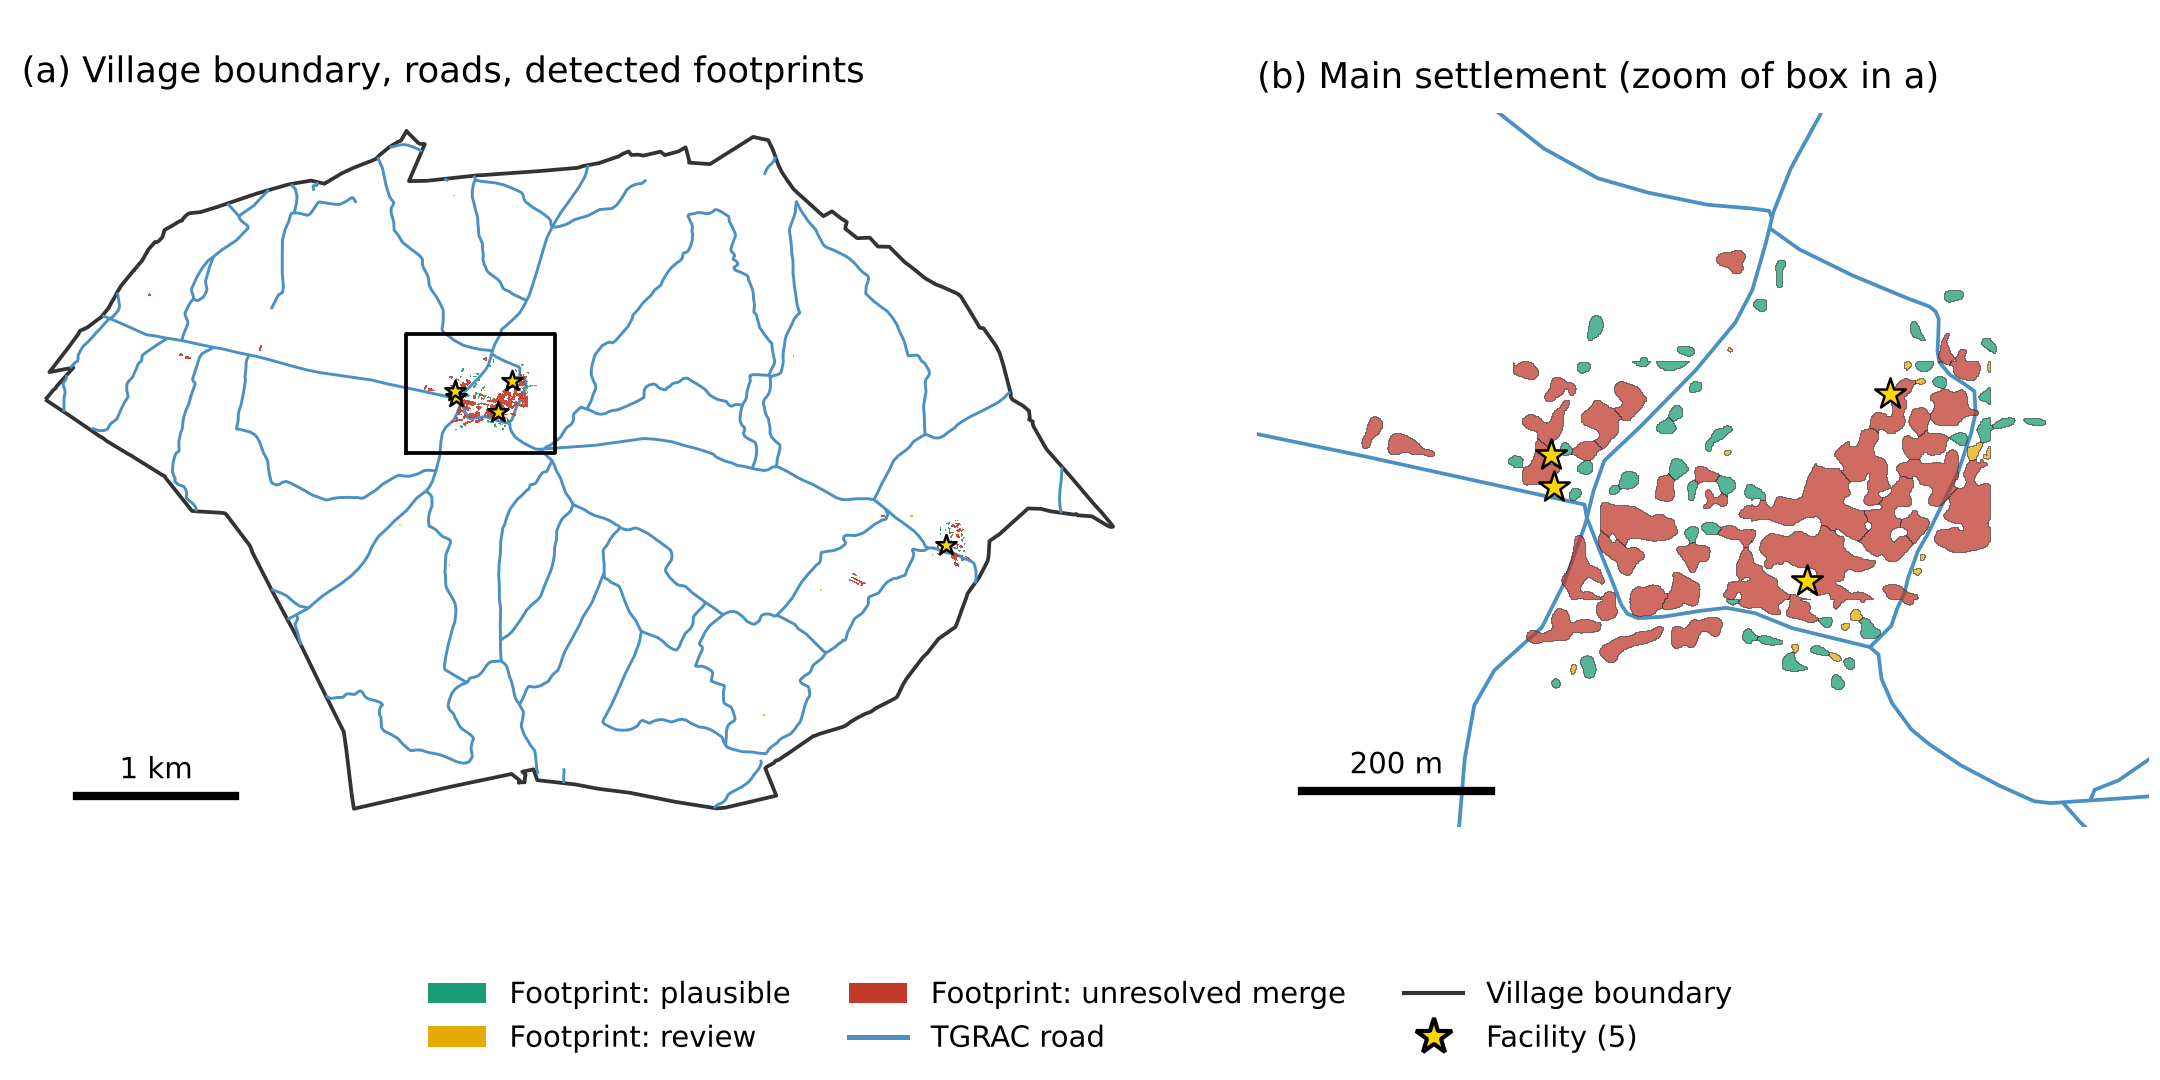
\includegraphics[width=\columnwidth]{figures/fig2_study_area.png}
\caption{Damarakunta. (a) Boundary, TGRAC roads and detected footprints by quality class, with the five facilities. (b) Main settlement. Footprints are automatic detections, not a census; no imagery basemap is shown because the imagery licence for derived products is unresolved.}
\label{fig:1}
\end{figure}

\subsection{Adilabad Urban (urban and peri-urban)}

The second window is the Adilabad Urban mandal, Adilabad district (geoBoundaries ADM3 polygon \cite{runfola2020geoboundaries}; centroid 19.682\textdegree{}N, 78.528\textdegree{}E), 17.75 km\textsuperscript{2}, close to Damarakunta in area. Its 10 m grid has 424 $\times$ 564 cells, 177,533 of them inside the polygon and 0.62\% blocked (water or slope above 25\textdegree{}). About 60\% of cells are not WorldCover built-up, so the window holds an urban core and a peri-urban fringe. The boundary is the 2018 release and may differ from current municipal limits.

All Adilabad layers are open (Table I). Overture release 2026-10-21.0 \cite{overture2026} supplies 4,850 road segments, 24,924 building polygons (18,846 from OpenStreetMap and 6,078 from Google Open Buildings v3 \cite{sirko2021openbuildings}) and 738 places. Footprints with area $\geq$ 30 m\textsuperscript{2} and confidence $\geq$ 0.7 (18,242 polygons) form the penalty layer. Of 107 school, health and government place candidates, 83 fall inside the window and 71 are verified (44 schools, 20 health, 7 government): records with mis-geocoded foreign place names were removed manually and a footprint within 20 m of the point was required. StrongDINOv2Seg was \textbf{not} run on Adilabad: the weights' location was not recorded, the Esri imagery licence for derived products is unresolved and no open sub-metre imagery was available. The Adilabad building layer is therefore open map data, not model output, and has not been field-verified.

\begin{table}[!t]
\caption{Input data and licence status}
\label{tab:1}
\centering
\scriptsize
\setlength{\tabcolsep}{2pt}
\begin{tabular}{>{\raggedright\arraybackslash}p{0.671in}>{\raggedright\arraybackslash}p{1.387in}>{\raggedright\arraybackslash}p{1.074in}}
\toprule
\textbf{Layer} & \textbf{Damarakunta / Adilabad source} & \textbf{Licence status} \\
\midrule
Boundary & TGRAC / geoBoundaries ADM3 & Not stated / ODbL 1.0 \\
Roads, facilities & TGRAC (43 road features, 5 facilities) / Overture 2026-10-21.0 & Not stated / ODbL 1.0 (roads), CDLA-Permissive-2.0 (places); not re-verified \\
Buildings & StrongDINOv2Seg candidates (0.6 m Esri imagery) / Overture footprints (OSM, Google Open Buildings v3) & Imagery licence for derived products unresolved / ODbL 1.0 and CC BY 4.0; not re-verified \\
Land cover & ESA WorldCover v200, 10 m \cite{zanaga2021worldcover} & CC BY 4.0 \\
Terrain & \textasciitilde{}30 m DEM (source not recorded) / Copernicus GLO-30 \cite{esa2022copdem}; Sobel slope, bilinear to 10 m & Not stated / as stated by provider \\
Training data & LoveDA \cite{wang2021loveda} & Source domain only \\
\bottomrule
\end{tabular}
\end{table}

\section{Methodology}

Fig. 2 summarises the architecture. The two settlements differ in the perception and target stages and share the cost surface, planner and evaluation stages.

\subsection{Semantic segmentation: StrongDINOv2Seg}

StrongDINOv2Seg uses the pre-trained facebook/dinov2-base encoder (DINOv2 ViT-B/14 \cite{oquab2023dinov2}), fully fine-tuned. Tokens from transformer blocks 3, 6, 9 and 12 are projected to 256 channels and fused in a feature-pyramid manner \cite{lin2017fpn}, passed through an atrous spatial pyramid pooling neck with rates 6, 12 and 18 \cite{chen2018deeplabv3plus} and a four-stage residual decoder with auxiliary heads for deep supervision \cite{lee2015dsn}. Training on LoveDA \cite{wang2021loveda} used 560 px inputs for a scheduled 10 epochs with AdamW, a cosine learning-rate schedule to 10\textsuperscript{-7}, an encoder learning rate of 0.1 times the base rate, and the loss 0.5$\cdot$CE + 0.4$\cdot$Dice + 0.1$\cdot$edge \cite{milletari2016vnet} with auxiliary weight 0.4. The epoch-4 checkpoint was evaluated and used.

\subsection{Instance extraction and facility verification}

Building instances are extracted from the predicted mask with OpenCV and NumPy. For each connected component, a Euclidean distance transform is computed; h-maxima, obtained by iterative morphological reconstruction with a 3 $\times$ 3 dilation, give one marker per candidate roof; a priority-driven marker-controlled flooding of the distance transform (a watershed-type transform) assigns pixels to markers; and adjacent pieces are merged back unless the saddle height between them is below 0.65 of the lower peak (neck test) and each piece exceeds a minimum area. Components that cannot be split reliably are flagged Unresolved\_Merge, and the remaining polygons are labelled Plausible or Review by size and shape rules. Facilities are accepted as targets only if they lie inside the boundary and have a detected footprint within 20 m of the recorded point; the same rule is applied to Overture places in Adilabad, together with manual removal of mis-geocoded records.

\subsection{Open-data mode and road-gap targets}

For Adilabad, Overture footprints replace the segmenter output. Because connecting every footprint is meaningless in a built-up fabric already served by roads, only houses more than 30 m (the planner snap distance) from an existing road are routed. Planner cost grows roughly quadratically with the number of targets, which further motivates the filter; the threshold is varied (20, 30, 50 m) in Section V-E.

\subsection{Multi-criteria cost surface}

Let \textit{B} be the set of blocked cells (water, invalid cells, slope above 25\textdegree{}) and \textit{P} the set of cells whose centre lies inside a footprint. The graph has the unblocked 10 m cells as nodes and 8-neighbour edges without diagonal corner-cutting. The cell cost is
\begin{equation}
c(x) = \bigl[\, c_{\mathrm{lc}}(\ell(x)) + g(s(x)) \,\bigr]\, m(x)
\label{eq:1}
\end{equation}

where \textit{m}(\textit{x}) = $\mu$ if \textit{x} $\in$ P and 1 otherwise, $\ell$ is the ESA WorldCover class \cite{zanaga2021worldcover} with resistances 8, 5, 3, 6, 2 and 4 for classes 10 (tree cover), 20 (shrubland), 30 (grassland), 40 (cropland), 50 (built-up) and 60 (bare/sparse), g(s) = 4$\cdot$clip(s, 0, 10)/10 with s the slope in degrees derived from the DEM \cite{esa2022copdem}, and $\mu$ = 4 is the footprint penalty. Edge weights are the mean end-cell cost times step length. The 25\textdegree{} slope limit is a project rule, not a transcription of Indian Roads Congress standards, and costs are ordinal planning units, not currency. In Damarakunta the penalty is lifted within a 20 m disc around the health sub-centre, whose point lies on the edge of its own footprint.

\subsection{Two-stage shared-network planner}

For each target, Stage A computes a least-cost path to the existing road cells with Dijkstra's algorithm \cite{dijkstra1959note,hart1968astar,collischonn2000lcp} and obtains alternatives by inflating costs along earlier paths (K = 3 alternatives in total). Stage B greedily selects the (target, alternative) pair with the highest weight per marginal cost
\begin{equation}
\Delta L_{\mathrm{cost}}(\pi \mid S) = \sum_{e \in \pi \setminus E_S} w(e)
\label{eq:2}
\end{equation}

where \textit{E}\textsubscript{S} is the set of already selected edges, so built edges are free and a route may end on another route. This is the shortest-path heuristic for Steiner trees \cite{kou1981steiner,mehlhorn1988steiner} on a penalised, land-cover-weighted graph with the road network as a free sub-tree; it carries no optimality guarantee. Two leaf re-routing passes follow. Snap distance is 30 m, search limit 1,500 m and attachment tolerance 15 m. Facilities are planned in a separate phase (script plan\_network\_v2.py).

\subsection{Baselines, scenarios and metrics}

Four baselines are compared: straight lines, independent least-cost routes, a length-only control (distance instead of cost surface) and a roads-only shared reference (routes may share edges only with the existing road network). The saving against independent routing is $\rho$ = (\textit{L}\textsubscript{ind} $-$ \textit{L})/\textit{L}\textsubscript{ind}, with \textit{L} the unique network length (shared edges counted once). Exposure is measured by the number of routes crossing another house's footprint and the route length inside other footprints. The footprint penalty is varied ($\mu$ $\in$ \{1, 4, 20, 100\}, with a variant in which footprints are buffered by 7.1 m). For omissions, a target set \textit{M} is removed from the targets and from the penalty layer (a missed detection is absent from both) and the planner re-run; random draws use seeds 1--5. Reported are coverage, unserved households, change in unique length and length per routed target. No monetary cost is computed: the repository holds no rupee-denominated estimates, and the PMGSY scheme \cite{pmgsy} is used only as planning context.

\begin{figure*}[!t]
\centering
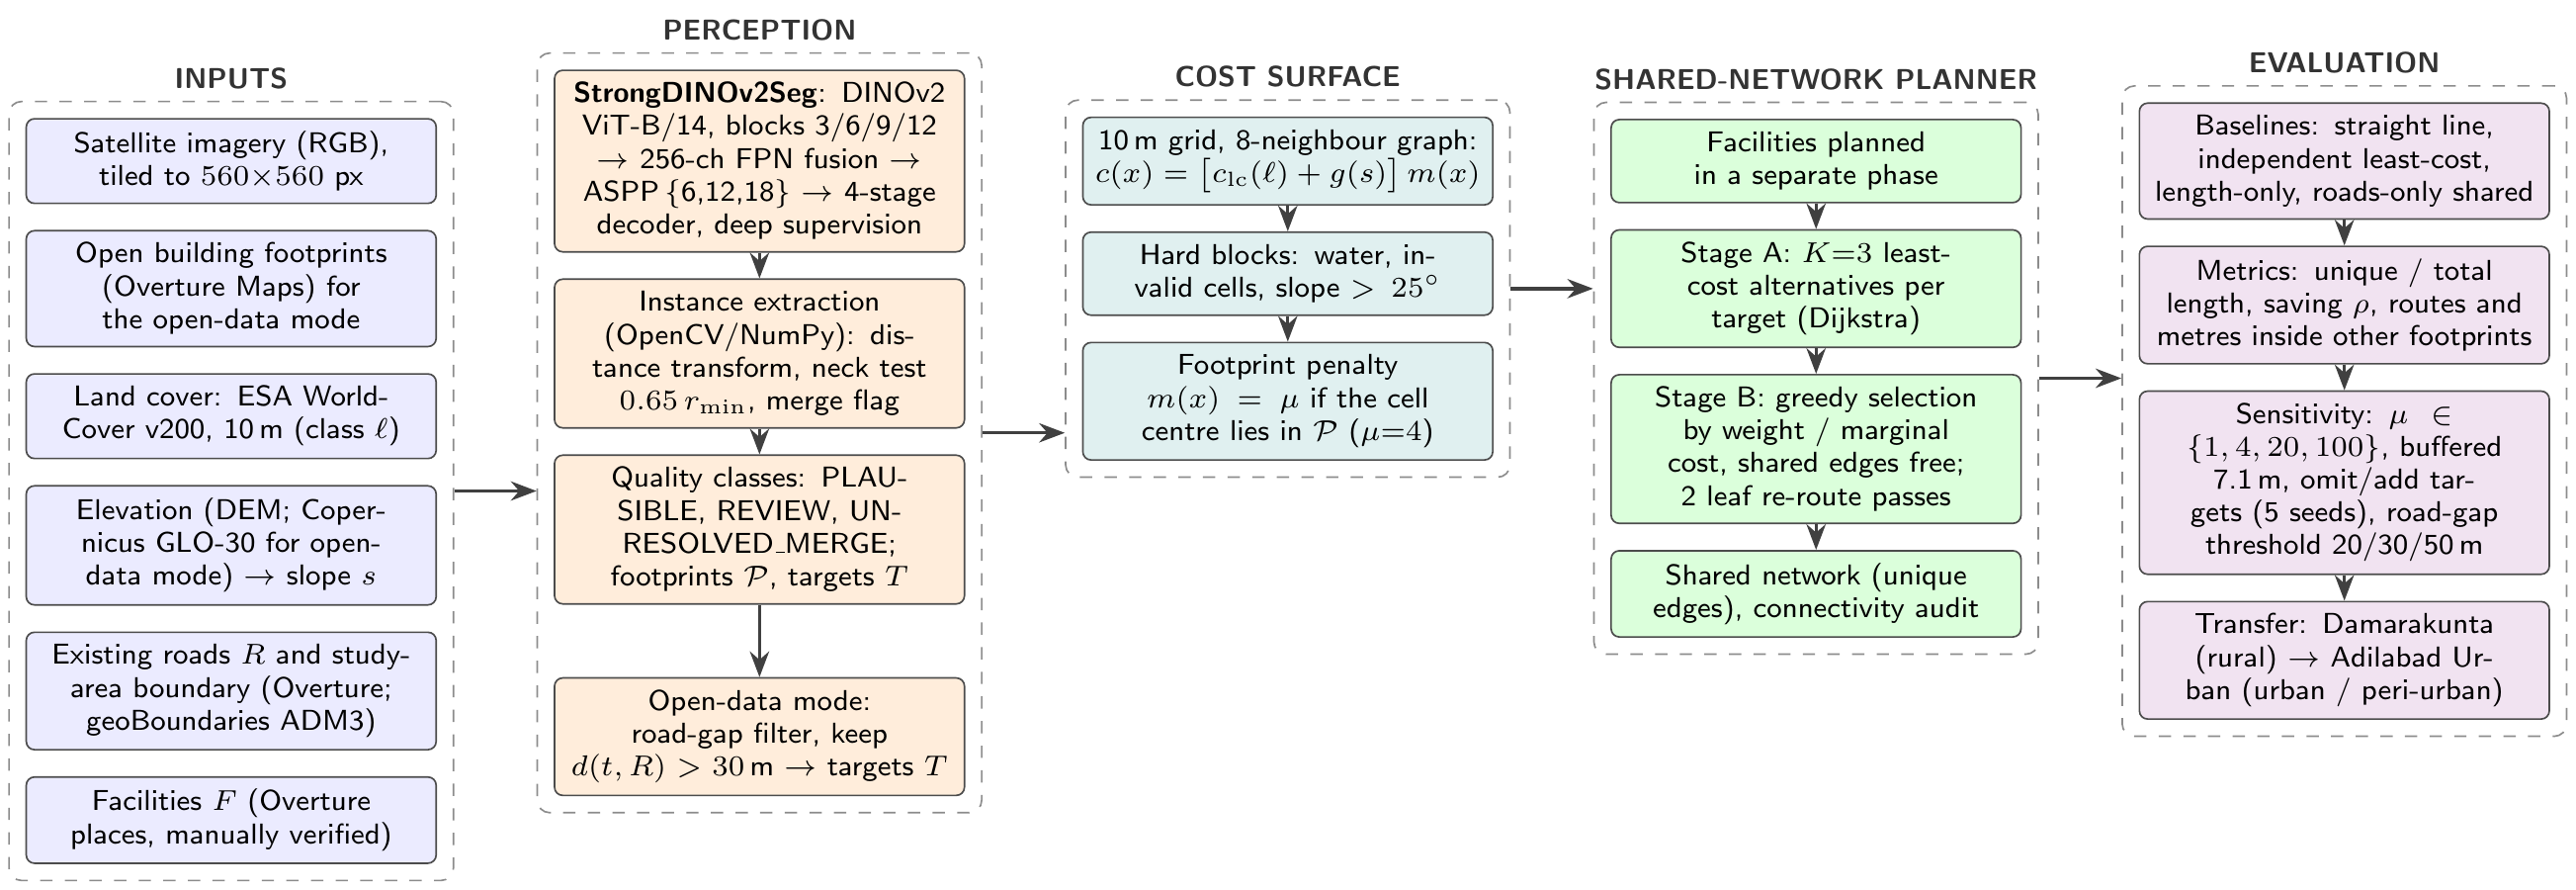
\includegraphics[width=0.98\textwidth]{figures/fig_architecture.png}
\caption{System architecture. Inputs feed a perception stage (Damarakunta: segmentation and instance extraction; Adilabad: open footprints enter the target stage directly with the road-gap filter), a shared cost surface, a two-stage shared-network planner and an evaluation stage that includes the cross-settlement transfer.}
\label{fig:2}
\end{figure*}

\section{Experiments and Results}

\subsection{Detection}

On the 1,669-image LoveDA validation split (560 px, seven scored classes) the epoch-4 checkpoint reached 53.8\% mIoU, 68.9\% Dice and 71.3\% pixel accuracy (recomputed from the saved confusion matrix), with 72.4\% macro precision and 66.9\% macro recall; for the Building class IoU is 54.0\%, precision 62.1\% and recall 80.6\% (Table II). These are source-domain figures, not accuracy on Damarakunta. Against Google Open Buildings v3 as a proxy (not ground truth), 118 of the 165 in-boundary candidates agree (71.5\%).

\begin{table}[!t]
\caption{Detection evaluation (LoveDA validation, \%; and proxy agreement)}
\label{tab:2}
\centering
\scriptsize
\setlength{\tabcolsep}{2pt}
\begin{tabular}{>{\raggedright\arraybackslash}p{1.034in}>{\raggedleft\arraybackslash}p{0.345in}>{\raggedleft\arraybackslash}p{0.362in}>{\raggedleft\arraybackslash}p{0.448in}>{\raggedleft\arraybackslash}p{0.388in}>{\raggedleft\arraybackslash}p{0.388in}}
\toprule
 & \textbf{mIoU} & \textbf{Dice} & \textbf{Pix. acc.} & \textbf{Prec.} & \textbf{Rec.} \\
\midrule
StrongDINOv2Seg & 53.8 & 68.9 & 71.3 & 72.4 & 66.9 \\
  Building class & 54.0 & 70.1 & --- & 62.1 & 80.6 \\
\multicolumn{6}{@{}l}{\textit{Damarakunta candidates vs. Open Buildings v3}} \\
Class & n & Agree & Disagree & Agr. \% &  \\
All & 165 & 118 & 47 & 71.5 &  \\
Plausible & 71 & 51 & 20 & 71.8 &  \\
Review & 32 & 14 & 18 & 43.8 &  \\
Unresolved\_Merge & 62 & 53 & 9 & 85.5 &  \\
\bottomrule
\end{tabular}
\end{table}

\subsection{Damarakunta: shared network and footprint penalty}

Independent least-cost routes for the 163 houses total 10,045.4 m, but because neighbouring houses re-trace the same corridors the unique built length is 6,753.1 m (Table III). The two-stage plan reduces this to 5,069.0 m, a saving of 24.9\%; all 163 houses and five facilities are connected. The length-only control has 3.4\% more unique length than independent cost-surface routing, and the roads-only shared reference saves 22.6\%, so most of the saving comes from sharing and a further 2.3 percentage points from sharing among new routes.

The penalty trades length for exposure (Fig. 3). With $\mu$ = 1 the plan is shortest (4,705.4 m) but 56 routes pass through other houses (660.1 m inside footprints). With $\mu$ = 4 it is 7.7\% longer while crossings halve to 28 routes and 209.1 m. Buffering footprints by 7.1 m with $\mu$ = 20 or 100 lowers crossings to 19 routes at 6,238.1 m and 6,190.3 m.

\begin{table}[!t]
\caption{Damarakunta routing, 163 houses ($\mu$ = 4 unless stated)}
\label{tab:3}
\centering
\scriptsize
\setlength{\tabcolsep}{2pt}
\begin{tabular}{>{\raggedright\arraybackslash}p{1.016in}>{\raggedleft\arraybackslash}p{0.423in}>{\raggedleft\arraybackslash}p{0.423in}>{\raggedleft\arraybackslash}p{0.339in}>{\raggedleft\arraybackslash}p{0.296in}>{\raggedleft\arraybackslash}p{0.466in}}
\toprule
\textbf{Strategy} & \textbf{Total (m)} & \textbf{Unique (m)} & \textbf{$\rho$ (\%)} & \textbf{Cross.} & \textbf{In fp. (m)} \\
\midrule
Straight line (2 infeasible) & 8,092.3 & --- & --- & 60 & 1,453.2 \\
Independent least-cost & 10,045.4 & 6,753.1 & 0.0 & 46 & 328.3 \\
Length-only control & 9,166.3 & 6,979.8 & $-$3.4 & 64 & 1,615.8 \\
Roads-only shared ref. & 5,229.3 & 5,229.3 & 22.6 & 29 & 216.1 \\
\textbf{Two-stage plan (proposed)} & \textbf{5,069.0} & \textbf{5,069.0} & \textbf{24.9} & \textbf{28} & \textbf{209.1} \\
\multicolumn{6}{@{}l}{\textit{No footprint penalty ($\mu$ = 1)}} \\
Independent least-cost & 9,595.9 & 6,921.3 & 0.0 & 63 & 1,423.1 \\
Two-stage plan & 4,705.5 & 4,705.4 & 32.0 & 56 & 660.1 \\
\multicolumn{6}{@{}l}{\textit{Buffered footprints (7.1 m), two-stage}} \\
Penalty $\mu$ = 20 & --- & 6,238.1 & 18.5 & 19 & 147.9 \\
Penalty $\mu$ = 100 & --- & 6,190.3 & 18.9 & 19 & 144.8 \\
\bottomrule
\end{tabular}
\end{table}

\begin{figure}[!t]
\centering
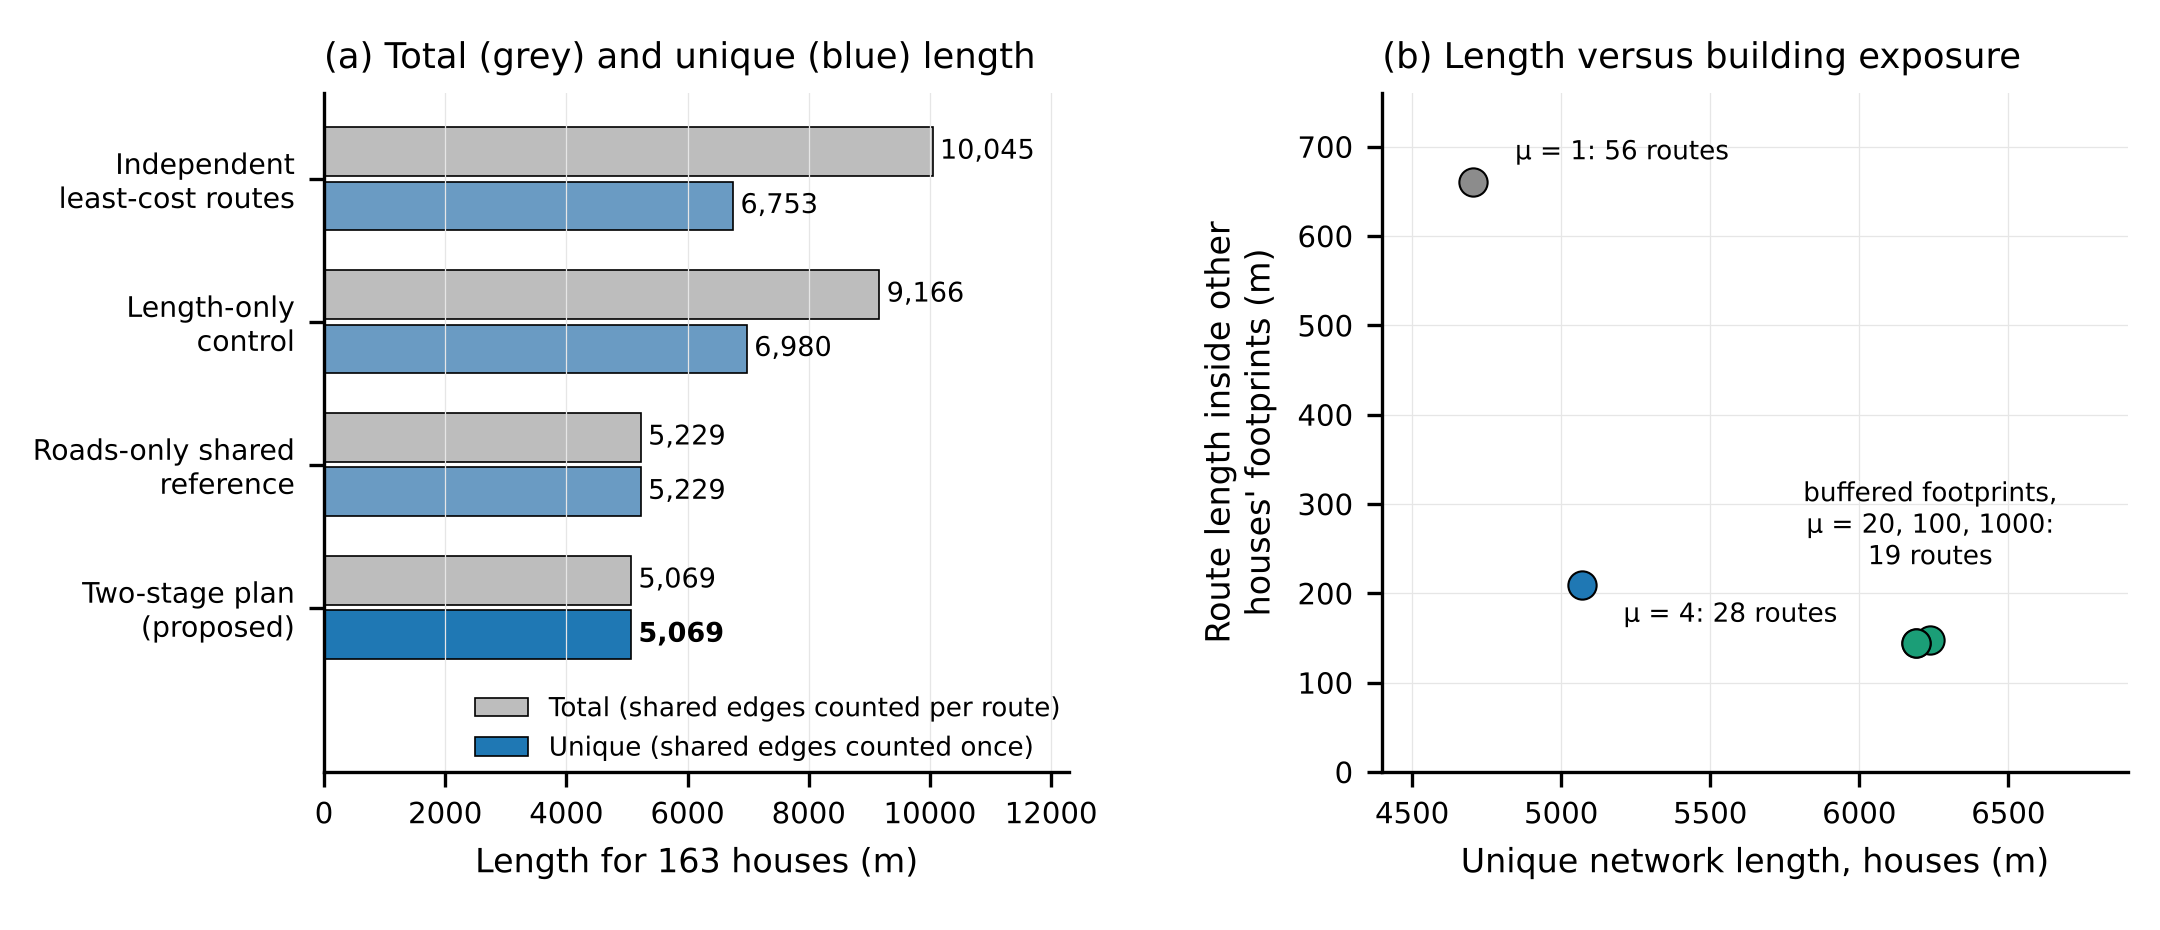
\includegraphics[width=\columnwidth]{figures/fig3_routing.png}
\caption{Damarakunta routing results for 163 houses. (a) Total and unique corridor length by strategy. (b) Unique network length against route length inside other houses' footprints for $\mu$ = 1, $\mu$ = 4 and buffered footprints with large penalties.}
\label{fig:3}
\end{figure}

\subsection{Damarakunta: impact of building omissions}

Table IV and Fig. 4 give the omission analysis against the 5,069.0 m baseline. Missing buildings make the plan \textit{shorter}: 10\% random omission (16 houses) understates length by 7.6\%, 20\% by 16.9\%, omission of the smallest quarter by 25.1\% and omission of all merged blobs by 29.4\%. At the same time U households lose access: 16 and 33 for random 10\% and 20\% omission, 41 for the smallest quarter and 62 (38.0\%) for merged blobs. A planner reading only total length would therefore underfund the scheme. Random additions lengthen the plan by 8.6\% and 15.8\%. The saving $\rho$ stays within 24.9--26.6\% across omissions, so the benefit of sharing is robust to inventory error.

\begin{table}[!t]
\caption{Simulated omissions and additions, Damarakunta (baseline 5,069.0 m, 163 routed)}
\label{tab:4}
\centering
\scriptsize
\setlength{\tabcolsep}{2pt}
\begin{tabular}{>{\raggedright\arraybackslash}p{0.929in}>{\raggedleft\arraybackslash}p{0.363in}>{\raggedleft\arraybackslash}p{0.242in}>{\raggedleft\arraybackslash}p{0.323in}>{\raggedleft\arraybackslash}p{0.404in}>{\raggedleft\arraybackslash}p{0.363in}>{\raggedleft\arraybackslash}p{0.283in}}
\toprule
\textbf{Scenario} & \textbf{Routed} & \textbf{U} & \textbf{$\kappa$ (\%)} & \textbf{L (m)} & \textbf{$\delta$\textsubscript{L} (\%)} & \textbf{$\rho$ (\%)} \\
\midrule
Baseline & 163 & 0 & 100.0 & 5,069.0 & 0.0 & 24.9 \\
Omit 10\% (random) & 147.0 & 16 & 90.2 & 4,684.4 & $-$7.6 & 25.1 \\
Omit 20\% (random) & 130.0 & 33 & 79.8 & 4,211.5 & $-$16.9 & 24.9 \\
Omit smallest 10\% & 146 & 17 & 89.6 & 4,648.6 & $-$8.3 & 24.9 \\
Omit smallest 25\% & 122 & 41 & 74.8 & 3,798.3 & $-$25.1 & 25.6 \\
Omit merged blobs & 101 & 62 & 62.0 & 3,579.0 & $-$29.4 & 26.6 \\
Add 10\% (random) & 177.4 & --- & --- & 5,502.4 & +8.6 & 25.6 \\
Add 20\% (random) & 190.6 & --- & --- & 5,868.3 & +15.8 & 25.4 \\
\bottomrule
\end{tabular}
\end{table}

\begin{figure}[!t]
\centering
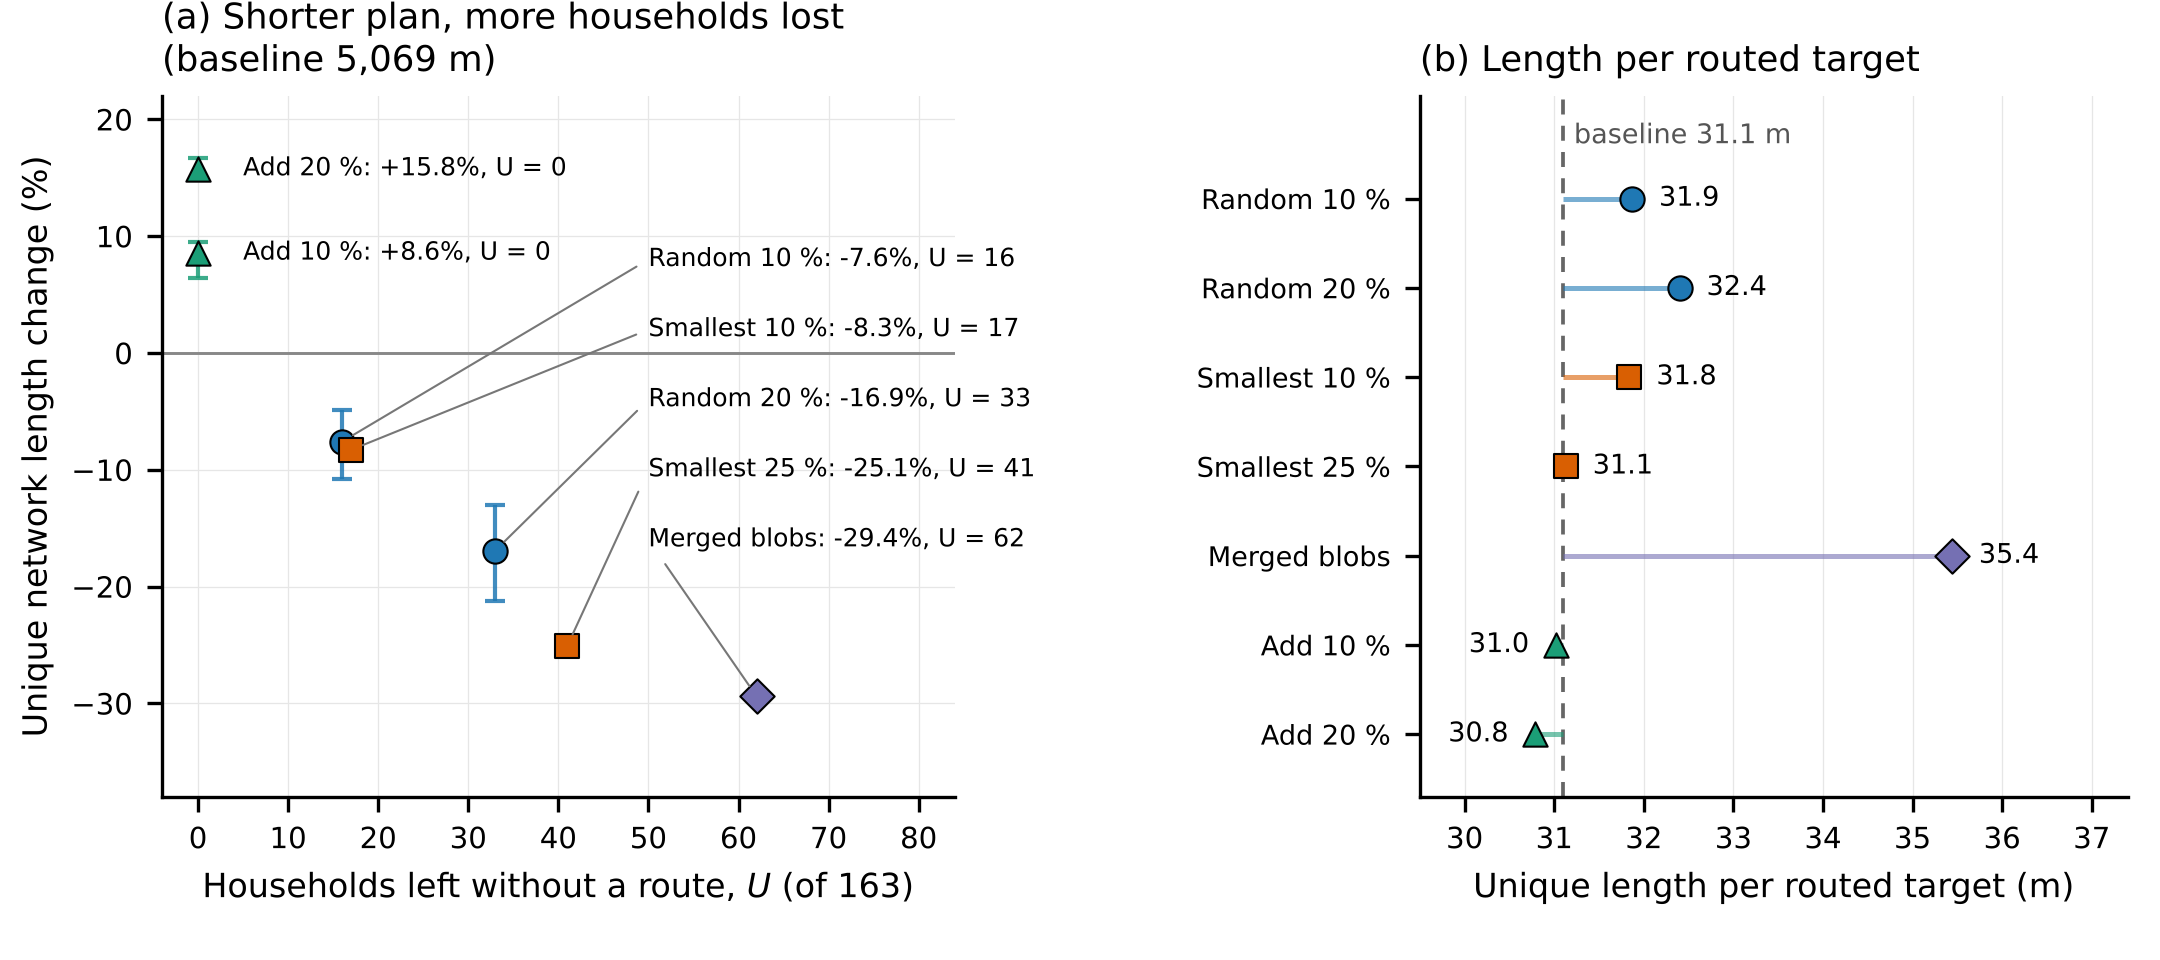
\includegraphics[width=\columnwidth]{figures/fig4_omission.png}
\caption{Damarakunta omission sensitivity (163 baseline targets; random scenarios are five draws with min--max bars). (a) Change in unique length against households left without a route. (b) Unique length per routed target.}
\label{fig:4}
\end{figure}

\subsection{Transfer to Adilabad Urban}

Of 18,242 penalty-layer footprints, 874 (4.8\%) lie more than 30 m from a road and form the targets; their median footprint is 139.6 m\textsuperscript{2} and median distance to the nearest road 42.3 m (Damarakunta: 235.8 m\textsuperscript{2} and 27.7 m). The planner routes 873 of 874. Independent least-cost routes total 56,308.0 m (unique 46,419.2 m); the two-stage plan needs 34,358.8 m, a saving of 26.0\% (Table V, Fig. 5). The facility phase connects 71 verified facilities with 1,090.1 m of unique corridor.

The baselines behave differently from the rural case. The roads-only shared reference saves just 2.9\% (22.6\% in Damarakunta) and the length-only control 5.7\% ($-$3.4\% in Damarakunta). In the dense fabric, targets are scattered among many existing roads, so sharing among \textit{new} routes accounts for almost all the gain, whereas in the dispersed village a trunk-and-branch structure off existing roads already captures most of it. Exposure is much higher: 332 of 873 routes (38\%) cross another footprint (2,041.1 m) against 28 of 163 (17\%) in Damarakunta.

\begin{table*}[!t]
\caption{Cross-settlement comparison under the same cost surface and solver}
\label{tab:5}
\centering
\footnotesize
\setlength{\tabcolsep}{2pt}
\begin{tabular}{>{\raggedright\arraybackslash}p{3.439in}>{\raggedleft\arraybackslash}p{1.624in}>{\raggedleft\arraybackslash}p{1.719in}}
\toprule
\textbf{Metric} & \textbf{Damarakunta (rural)} & \textbf{Adilabad (urban/peri-urban)} \\
\midrule
Study area (km\textsuperscript{2}) & 18.47 & 17.75 \\
House targets / routed & 163 / 163 & 874 / 873 \\
Independent routes, unique length (m) & 6,753.1 & 46,419.2 \\
Length-only control, unique (m) & 6,979.8 & 43,787.2 \\
Roads-only shared reference, unique (m) & 5,229.3 & 45,058.9 \\
\textbf{Two-stage plan, unique (m)} & \textbf{5,069.0} & \textbf{34,358.8} \\
Saving vs. independent (\%) & 24.9 & 26.0 \\
Roads-only shared saving (\%) & 22.6 & 2.9 \\
Unique length per routed house (m) & 31.1 & 39.4 \\
Routes crossing other footprints & 28 of 163 (17\%) & 332 of 873 (38\%) \\
Length inside other footprints (m) & 209.1 & 2,041.1 \\
$\mu$ = 1 $\rightarrow$ 4: unique length change (\%) & +7.7 & +13.3 \\
$\mu$ = 1 $\rightarrow$ 4: routes crossing & 56 $\rightarrow$ 28 & 618 $\rightarrow$ 332 \\
Facility phase: facilities / unique length (m) & 5 / 249.3 & 71 / 1,090.1 \\
10\% random omission: length change (\%) / unserved & $-$7.6 / 16 of 163 & $-$7.6 / 88 of 874 \\
20\% random omission: length change (\%) / unserved & $-$16.9 / 33 of 163 & $-$15.0 / 176 of 874 \\
Smallest-25\% omission: length change (\%) / unserved & $-$25.1 / 41 of 163 & $-$21.2 / 220 of 874 \\
\bottomrule
\end{tabular}
\end{table*}

\begin{figure*}[!t]
\centering
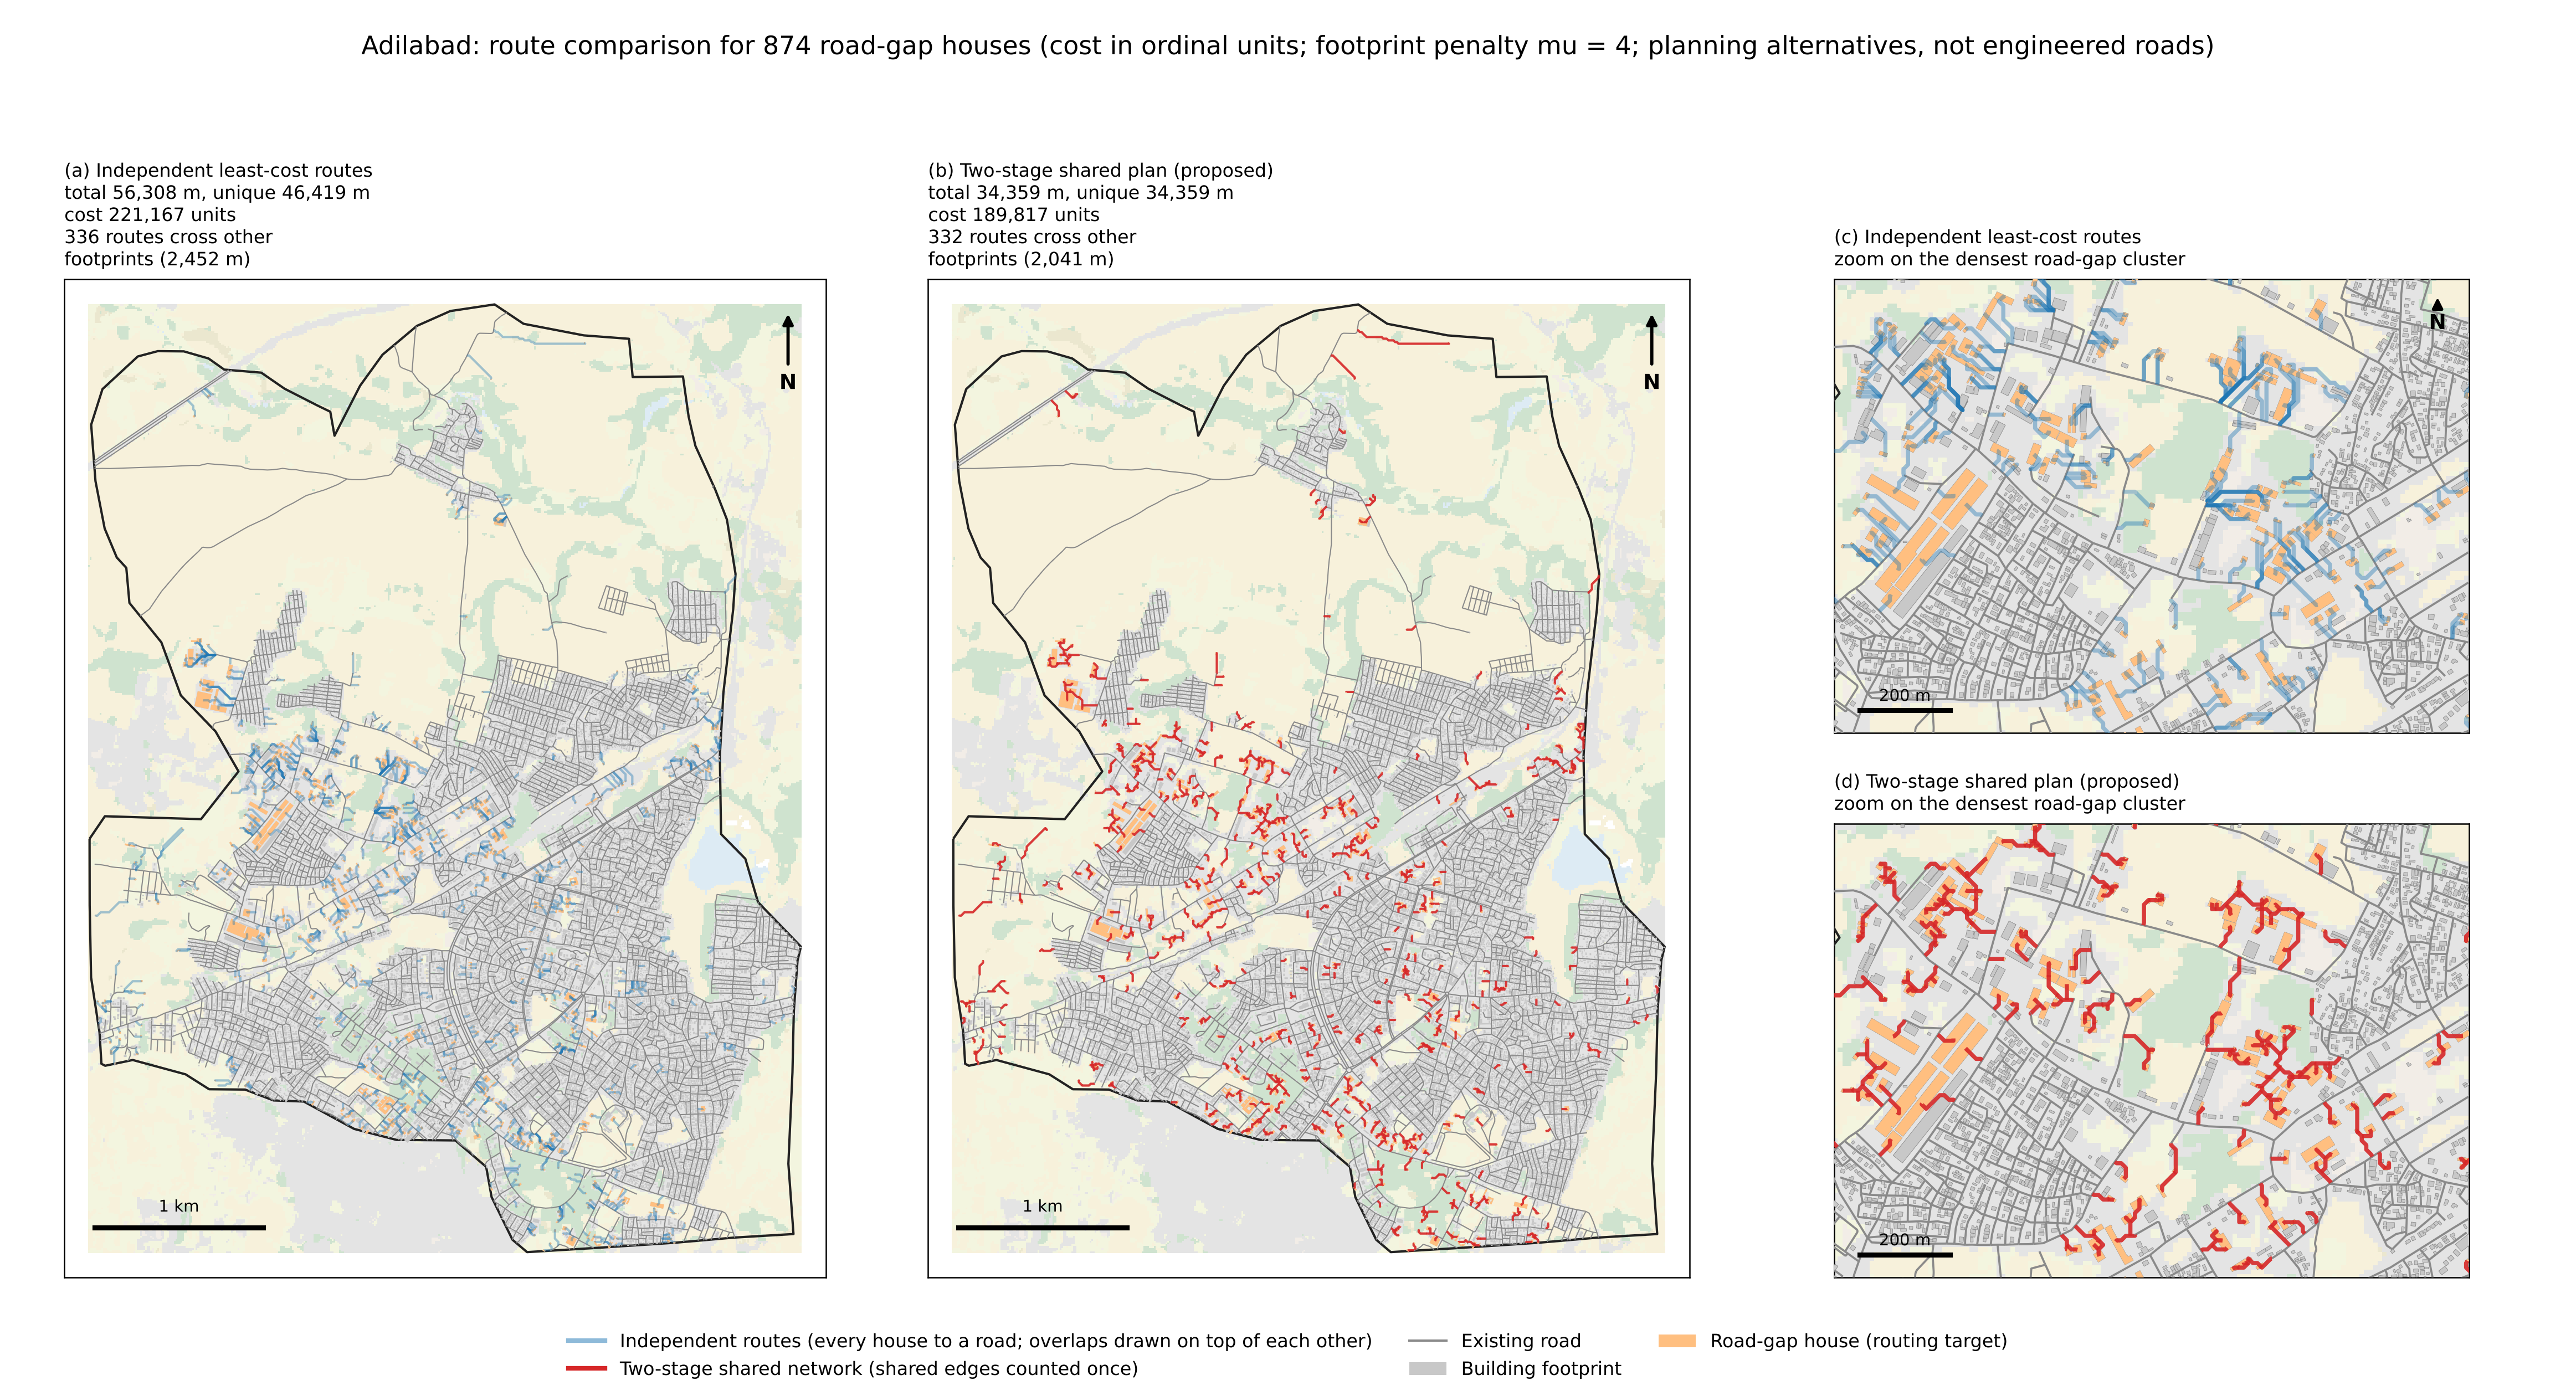
\includegraphics[width=0.98\textwidth]{figures/adilabad_map2_network_comparison.png}
\caption{Adilabad Urban route comparison for 874 road-gap houses ($\mu$ = 4): (a) independent least-cost routes, (b) two-stage shared plan, (c), (d) zoom on the densest road-gap cluster. Planning alternatives, not engineered roads; the basemap shows land cover and footprints only.}
\label{fig:5}
\end{figure*}

\subsection{Adilabad robustness}

\textit{Footprint penalty.} As in Damarakunta, raising $\mu$ from 1 to 4 lengthens the unique network by 13.3\% and removes 286 crossing routes (618 to 332). Settings $\mu$ = 20 and 100 give 37,024.1 m and 37,513.9 m with 271 and 275 routes crossing; buffered footprints give 42,071.9 m and 44,094.6 m with 231 and 221 crossing (Table VI, Fig. 6a). The saving against independent routing stays between 17.8\% and 30.8\% across all settings.

\textit{Road-gap threshold.} Defining targets as houses more than 20, 30 or 50 m from a road gives 2,190, 874 and 296 targets and savings of 21.9\%, 26.0\% and 29.5\%. The saving therefore depends on the target definition, which should be reported with any such result.

\textit{Omissions.} Random omission of 10\% and 20\% (five seeds) changes unique length by $-$7.6\% (range $-$8.9 to $-$6.7) and $-$15.0\% ($-$16.1 to $-$13.9), with 88 and 176 households unserved including one baseline failure; single-run smallest-10\% and smallest-25\% omissions give $-$7.9\% and $-$21.2\% (89 and 220 unserved). As in Damarakunta, missing buildings shorten the plan while stranding households, and the saving stays at 23.8--25.2\%. Merged-blob and addition scenarios were not defined for the open footprints.

\begin{table}[!t]
\caption{Adilabad sensitivity (874 targets unless stated)}
\label{tab:6}
\centering
\scriptsize
\setlength{\tabcolsep}{2pt}
\begin{tabular}{>{\raggedright\arraybackslash}p{1.313in}>{\raggedleft\arraybackslash}p{0.525in}>{\raggedleft\arraybackslash}p{0.350in}>{\raggedleft\arraybackslash}p{0.350in}>{\raggedleft\arraybackslash}p{0.481in}}
\toprule
\textbf{Setting} & \textbf{Unique (m)} & \textbf{$\rho$ (\%)} & \textbf{Cross.} & \textbf{In fp. (m)} \\
\midrule
Centre-in-footprint, $\mu$ = 1 & 30,335.7 & 30.8 & 618 & 4,893.0 \\
Centre-in-footprint, $\mu$ = 4 & 34,358.8 & 26.0 & 332 & 2,041.1 \\
Centre-in-footprint, $\mu$ = 20 & 37,024.1 & 22.8 & 271 & 1,687.4 \\
Centre-in-footprint, $\mu$ = 100 & 37,513.9 & 21.7 & 275 & 1,744.8 \\
Buffered 7.1 m, $\mu$ = 20 & 42,071.9 & 20.1 & 231 & 1,397.2 \\
Buffered 7.1 m, $\mu$ = 100 & 44,094.6 & 17.8 & 221 & 1,310.5 \\
Road-gap > 20 m (2,190 targets) & 65,204.4 & 21.9 & 815 & 4,543.9 \\
Road-gap > 30 m (874, primary) & 34,358.8 & 26.0 & 332 & 2,041.1 \\
Road-gap > 50 m (296 targets) & 15,880.9 & 29.5 & 126 & 809.9 \\
\bottomrule
\end{tabular}
\end{table}

\begin{figure*}[!t]
\centering
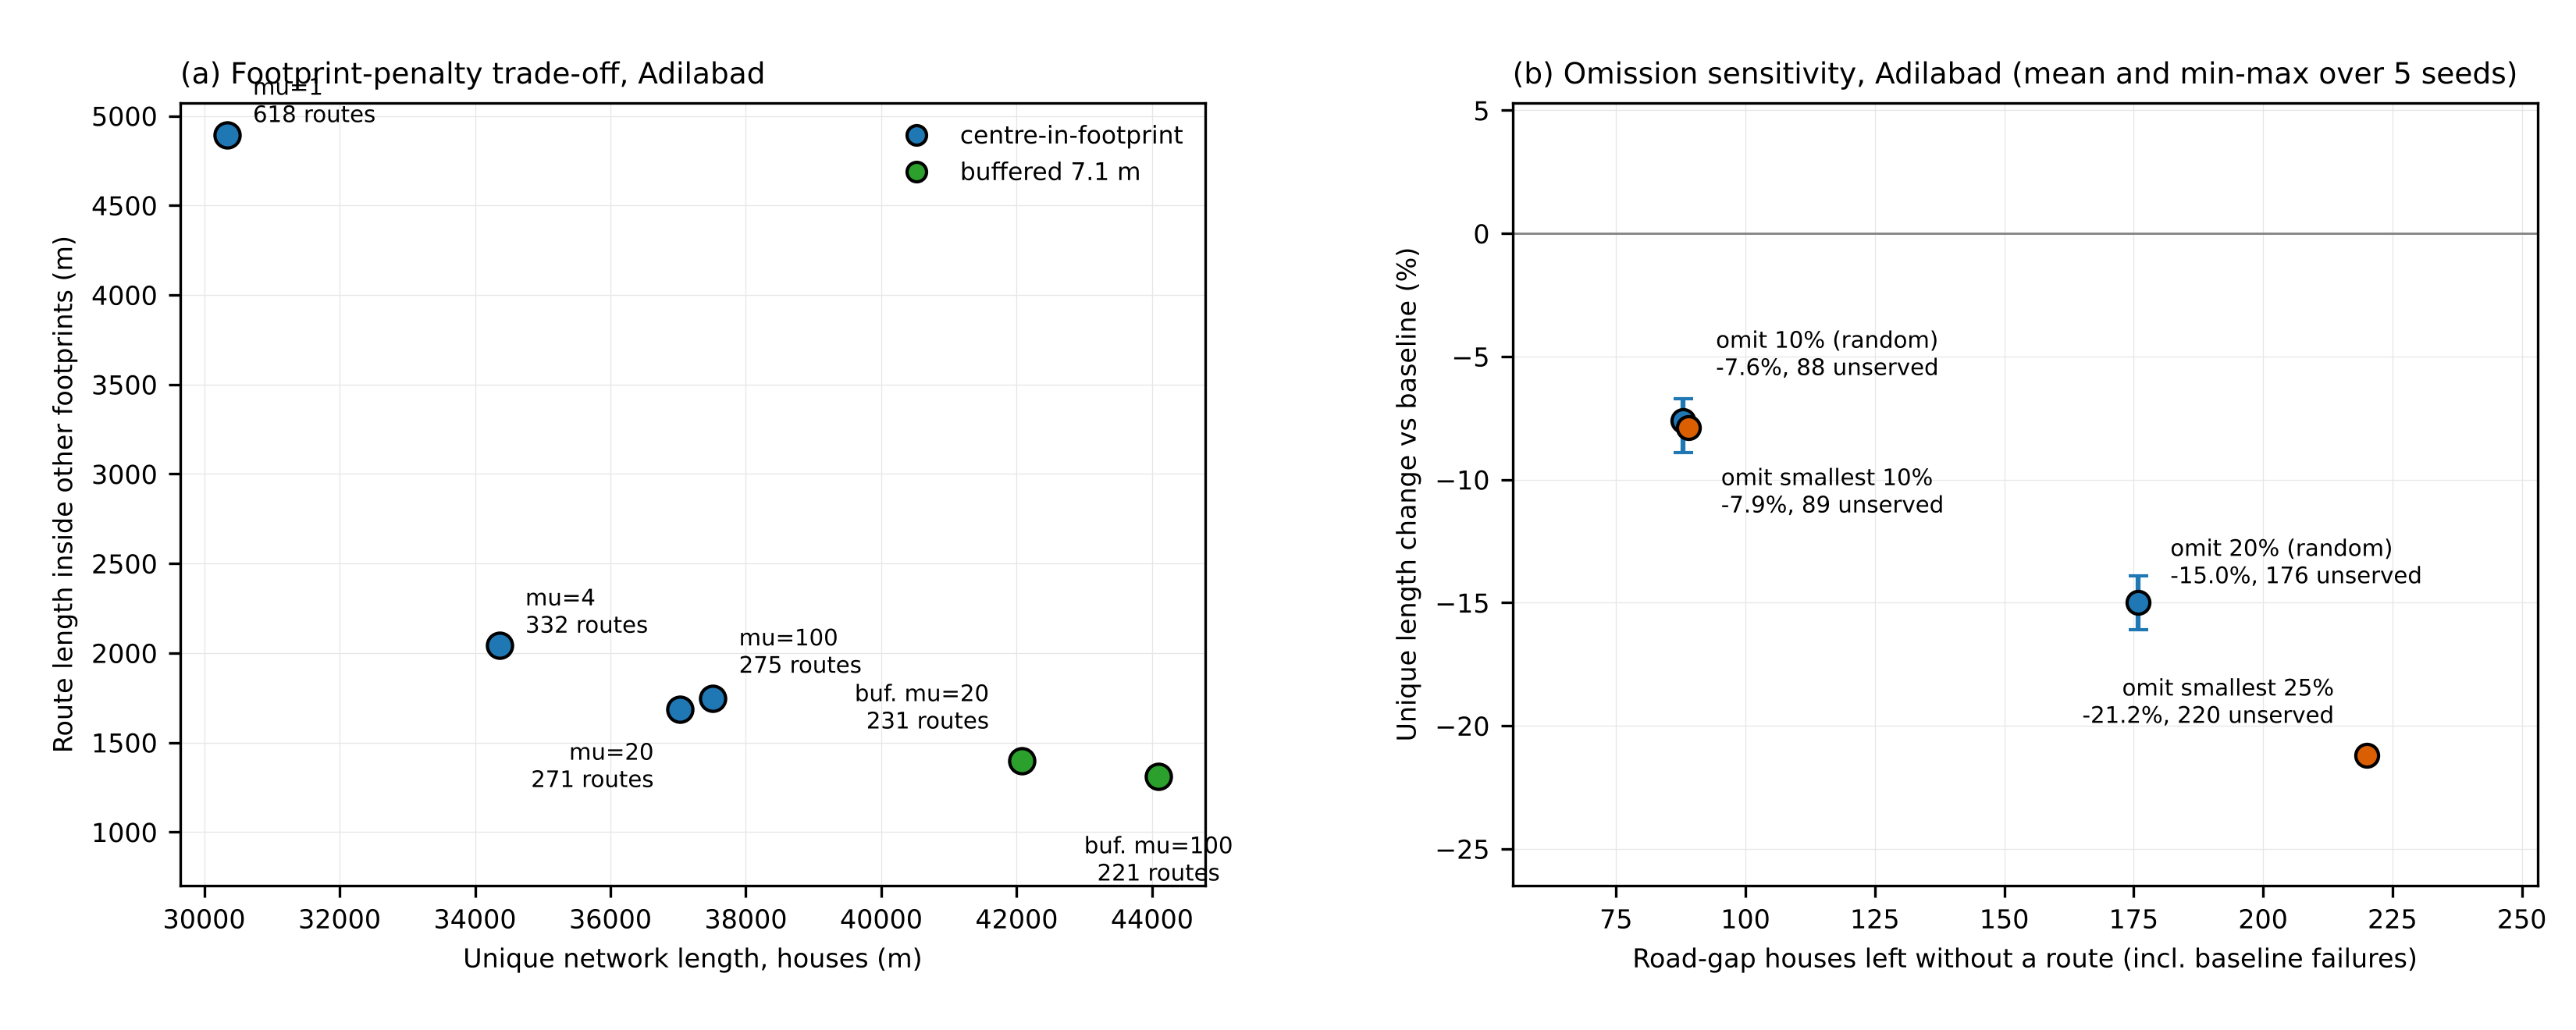
\includegraphics[width=0.98\textwidth]{figures/adilabad_fig3_sensitivity.png}
\caption{Adilabad sensitivity. (a) Footprint-penalty trade-off between unique network length and route length inside other footprints. (b) Omission sensitivity (random: mean and min--max over five seeds; smallest-q: single run).}
\label{fig:6}
\end{figure*}

\section{Discussion and Limitations}

\subsection{What transfers and what does not}

The planning stages transferred without modification: the same cost surface, solver parameters and metrics produced a connected plan in a window with more than five times as many targets (874 against 163), and the qualitative findings were reproduced: sharing saves about a quarter of the unique length (24.9\% and 26.0\%), the footprint penalty trades length for exposure, and omissions shorten the plan while stranding households. What did not transfer is the benefit of the simpler baselines: roads-only sharing recovered most of the gain in the dispersed village but almost none in the dense one. This suggests that the value of a marginal-cost planner grows with settlement density, a hypothesis supported by two settlements only. The effect of detection quality across settings could not be tested because Adilabad uses open map footprints.

\subsection{Why pixel metrics are not enough}

Segmentation metrics are area-weighted over classes, while the planner counts instances. A detector that misses the smallest quarter of buildings can lose few building pixels yet removes a quarter of the households from the plan (Table IV), and a detector that merges adjacent roofs can score a high pixel IoU yet strand 38\% of Damarakunta's houses in the merged-blob scenario. Network length falls in both cases, so total length is a poor quality indicator.

\subsection{Land take and planning use}

Shared corridors reduce new road length for the same households. As an illustration only, assuming a 5 m formation width (an assumption of this study; no road-width data were available), the 1,684 m saved in Damarakunta corresponds to about 0.84 ha less land take and the 12,060 m saved in Adilabad to about 6.0 ha. For PMGSY-style schemes \cite{pmgsy}, building inventories should be treated as uncertain inputs, with a sensitivity band on any network sized from them. The outputs are screening-level alternatives; no compliance with Indian Roads Congress design standards and no cost in rupees is claimed.

\subsection{Limitations}

(i) Two settlements only; the semi-urban and second rural windows are planned but not run. (ii) Omission scenarios are synthetic, not measured detection errors. (iii) Damarakunta has no surveyed reference; the LoveDA metrics come from the epoch-4 checkpoint with metadata recovered from the training notebook, and the checkpoint hash was not logged with the village candidates. (iv) Adilabad footprints are open map data of unverified completeness and the Overture licences were not re-verified. (v) Costs are ordinal, the planner is a heuristic without an optimality guarantee, and road-gap targeting changes the problem, as the threshold sweep shows. (vi) Pixel accuracy is reported as 71.3\%, the value recomputed from the confusion matrix.

\section{Conclusion}

A pipeline from satellite imagery and open layers to shared access roads connects the houses and facilities of a rural village with 24.9\% less unique corridor than independent routing and, without changes to the cost surface or solver, those of an urban and peri-urban mandal with 26.0\% less. Footprint penalties and simulated inventory errors behave consistently in both settings: penalties trade length for fewer routes through dwellings, and omissions shorten the plan while stranding households. The dependence of the roads-only baseline on settlement density and the effect of detection quality across settings are the main open questions; a semi-urban and a second rural window are planned to address the first.

\section*{Acknowledgment}

The authors acknowledge the Telangana State Remote Sensing Application Centre (TGRAC) for the Damarakunta boundary, road and facility layers, and the providers of the open datasets used (ESA WorldCover, Copernicus DEM, Overture Maps, geoBoundaries, Google Open Buildings, LoveDA). This research received no specific grant from any funding agency in the public, commercial, or not-for-profit sectors. The authors declare no competing interests.

\section*{Data Availability}

Code, derived summary tables and open-data manifests with SHA-256 hashes are available at https://github.com/Archana519/Telangana-Rural-Project (folders DELIVERABLES\_DAMARAKUNTA\_STAGE\_B and DELIVERABLES\_CONTRIBUTION\_3\_MULTI\_VILLAGE). TGRAC layers are subject to the provider's terms; Esri imagery is not redistributed. A Zenodo DOI will be added when the archive is minted.

\bibliographystyle{IEEEtran}
\bibliography{references}
\end{document}
